This chapter summarises the goals of the content profiling approach discussed so far and gives a detailed overview of the architecture for a prototype implementation of it. First a high-level design is discussed and then detailed explanation of the chosen technology, trade-offs, implementation details and enhancements made is provided. Afterwards some algorithms for representative sample selection that were implemented are presented and discussed. At the end a short summary and overview of future interesting work which will enhance the tool and help preservation experts even more in their endeavours is given.

\section{C3PO in Perspective}
As part of this thesis, a software prototype is developed that aims to tackle the issues, problems and gaps presented in the previous chapters. The aim is to create a tool that is able to automatically generate a content profile of large collections (consisting of hundreds of thousands, or even millions of objects). This means a framework that provides enough scalability to be feasibly applied on the metadata of collections of multi-terabyte ranges and beyond.

This profile includes a descriptive statistical representation of the content in the collection, meaning that it contains very specific data such as count of objects, overall size of objects, etc. Furthermore, it provides visualisations of different aspects of the content, such as the file formats, mime types and many other characteristics and combinations thereof that are of interest to the user of the application.

As presented in section \ref{sec:goals} on page \pageref{sec:goals}, the tool that implements the presented approach should fulfil the following requirements.

\begin{description}
\item[R1] The user should be able to aggregate large sets of meta data.
\begin{description}
\item[R1.1] This should happen with minimal effort spent for setup and configuration and happen in an automated fashion.
\item[R1.2] The process should finish in a time frame short enough, so that the information in the generated profile is
still up to date.
\item[R1.3] The time needed for the process to finish should scale linearly to the size and volume of the collection.
\end{description}
\item[R2] The presented approach should scale up to a million objects and should be ready to pass this threshold by making use of a distributed infrastructure and architecture.
\item[R3] Clients of the application (users, or other systems) should be able to obtain a machine-readable description of the profile, that contains an overview of the content at hand.
\begin{description}
\item[R3.1] This profile shall include the identifiers of a small set of objects that are representative to the whole collection, as described in section \ref{sec:representative_sets} on page \pageref{sec:representative_sets}.
\item[R3.2] The profile shall include an identifier of the collection as well as the object identifiers it refers to.
\end{description}
\item[R4] Planning experts should have the ability to visualise different aspects of the content.
\item[R5] Planning experts should have the ability to filter the content based on chosen characteristics.
\item[R6] Planning experts should have the ability to present the raw meta data or a subset of it in a sparse matrix view, where each row is a digital object, each column is a property, and each cell has the value of the corresponding property for the corresponding element.
\end{description}

%On top of that a service layer enables the user to query the tool in order to gain a deeper insight into the content. This may include the filtering of the content based on different characteristics and splitting it into buckets, which will allow to compare homogeneous parts (based on one or more characteristika) in an otherwise heterogenous content. 

%Visualizations and multi dimensional representations of these filterings enable to user to understand the profile and thus provide her with the fundamental knowledge and a more stable ground to take more efficient decisions.
The prototype implementation of the profiling approach is called '\textbf{C}lever, \textbf{C}rafty \textbf{C}ontent \textbf{P}rofiling of \textbf{O}bjects' or \textit{C3PO} for short and is discussed in detail in the following subsections.
% idea
% overview
% part of scape, watch source, etc..

\section{Architecture}
In this section an overview of the architecture of C3PO is presented. Afterwards, detailed information about the design and implementation is given as well as a discussion of the decisions made is done. The implementation was carried out in two iterations, which are presented after the overview.

\subsection{High Level Overview}
C3PO is separated into different modules and provides a relatively simple workflow that follows the three steps of content profiling as presented in \cite{petrov-ipres2012} and discussed in section \ref{sec:content_profiling}. In the first part, it gathers raw meta data and parses it in order to normalise it into a simple internal data model. In the next step, the data is cleaned up, partially aggregated and stored into a database.

All this offers the baseline for the deeper analysis provided by some of the modules of the framework. Figure \ref{fig:architecture_highlevel} presents the high level architecture and C3PO's modules in a stack diagram that is detailed in the following subsections.


\begin{figure}[t]
\begin{center}
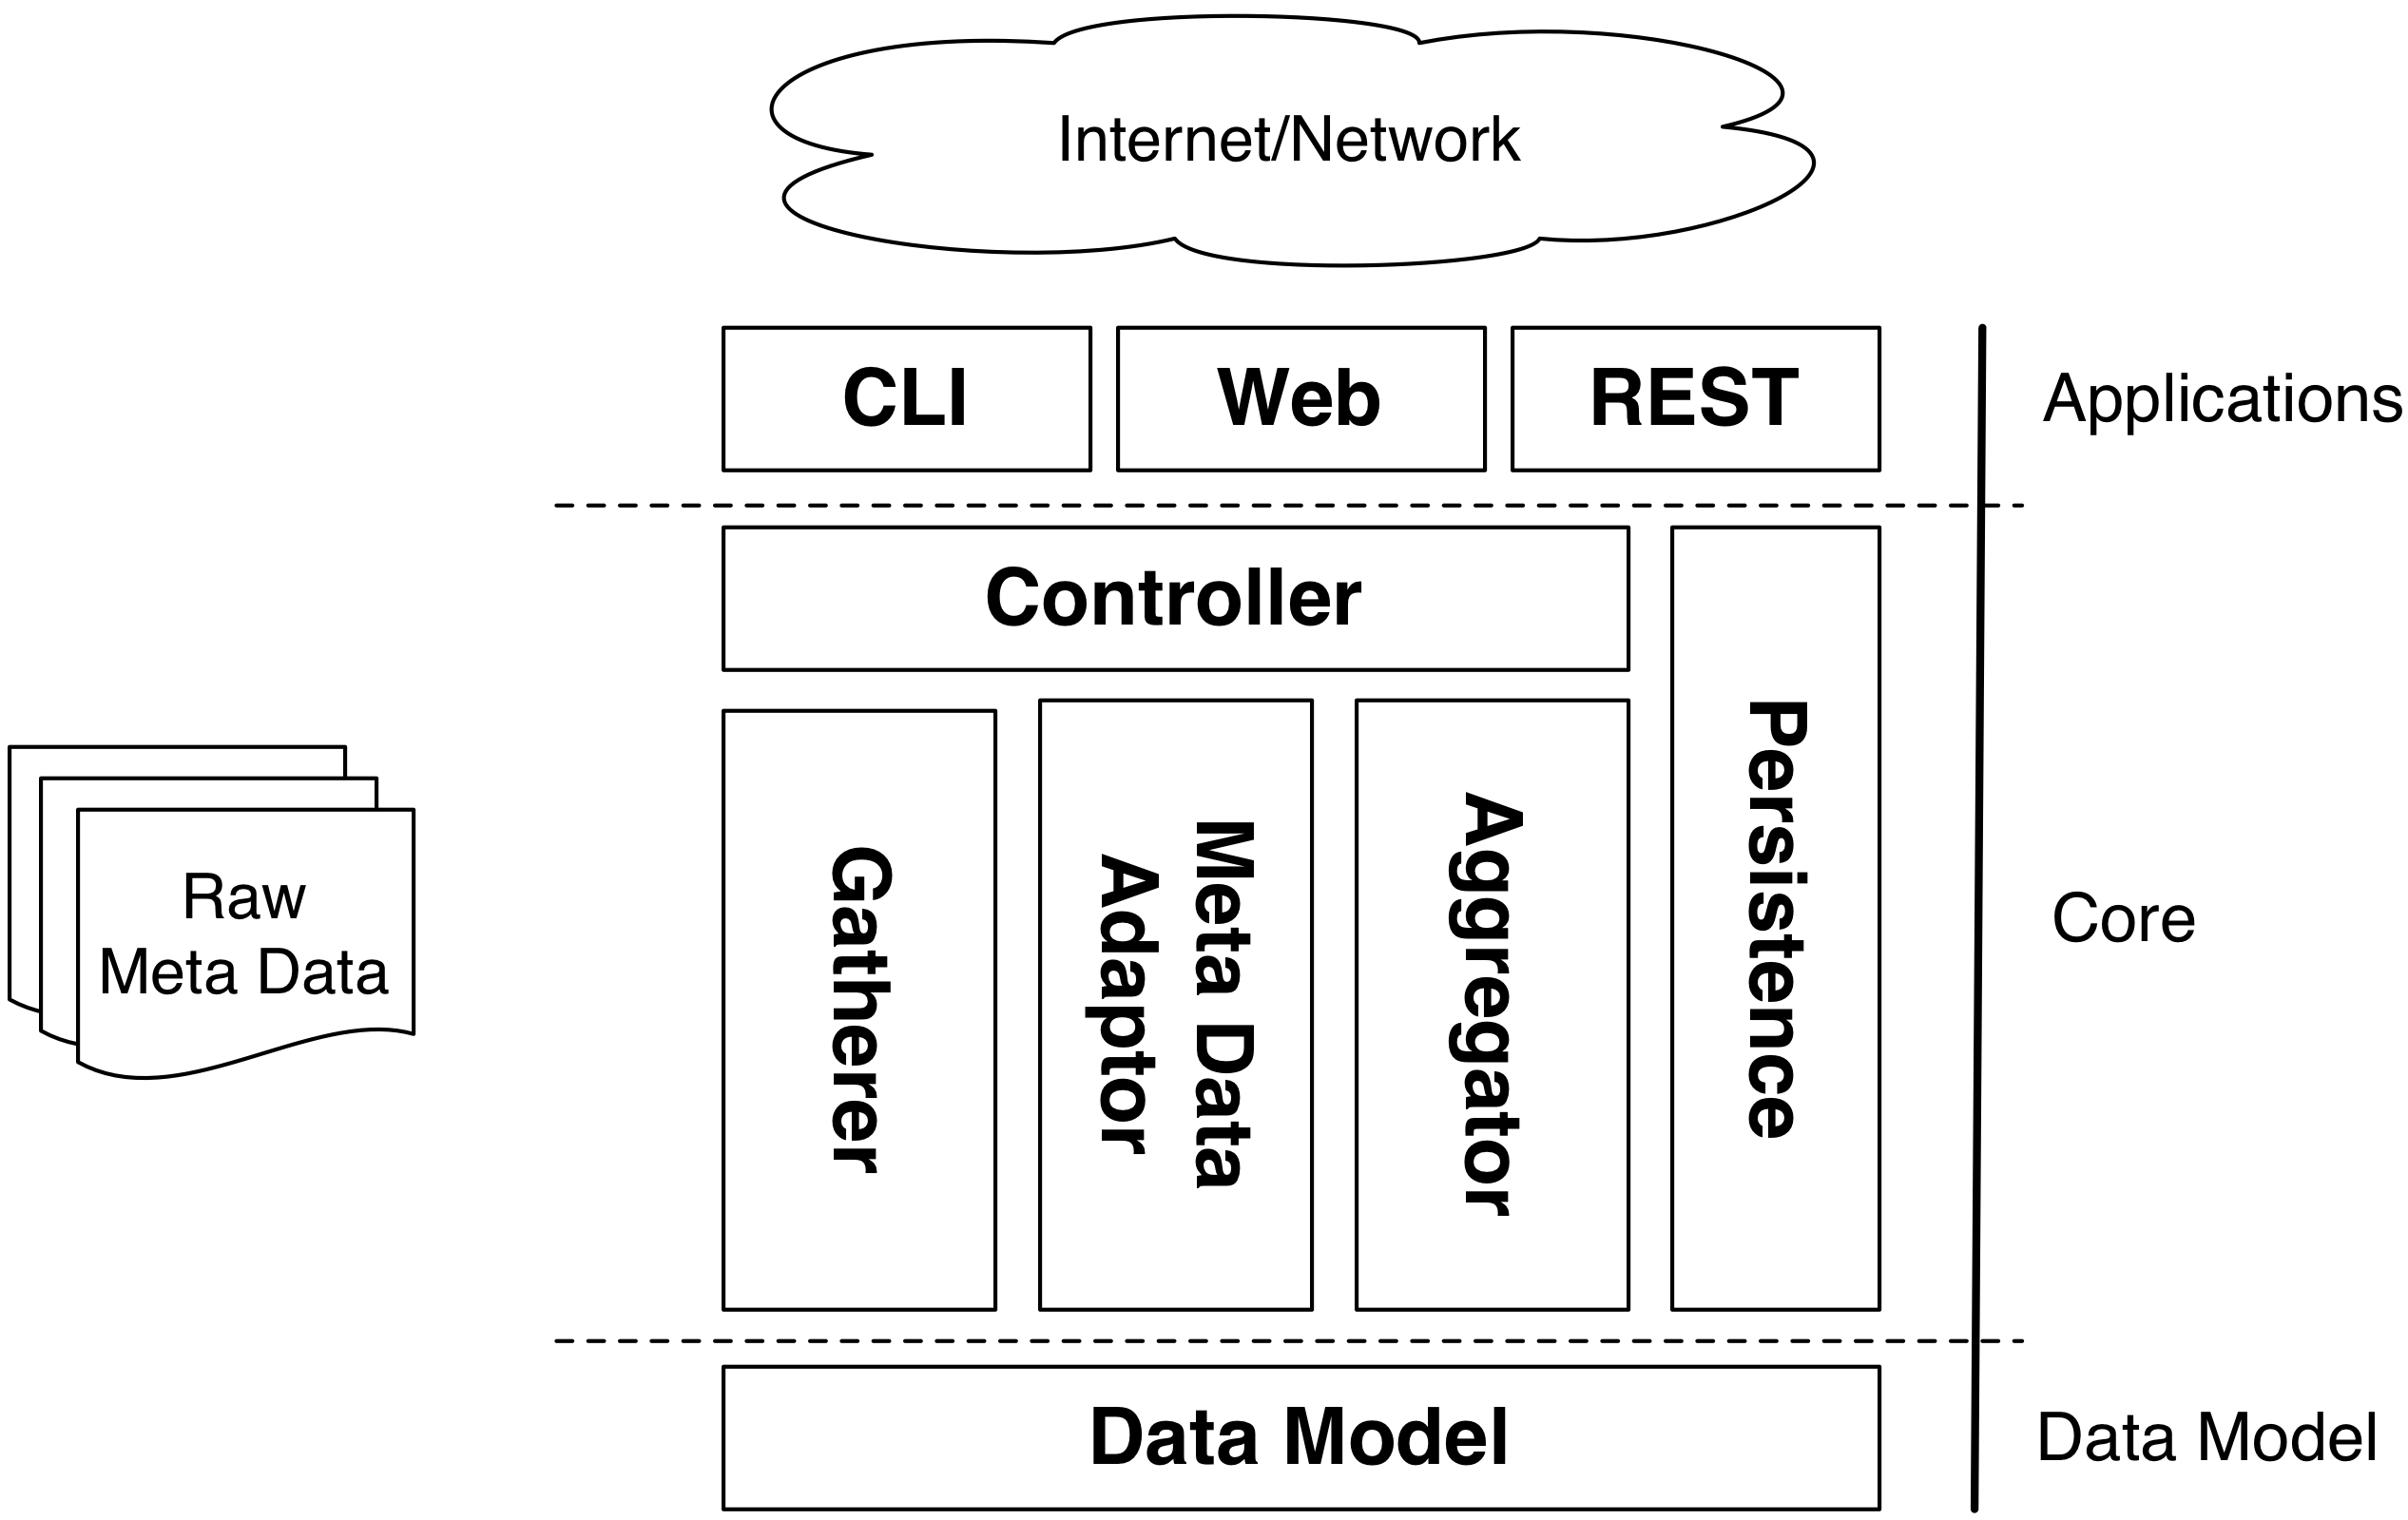
\includegraphics[width=5in]{figures/architecture/c3po_highlevel_architecture.png}
\caption{High-level architecture of C3PO.}
\label{fig:architecture_highlevel}
\end{center}
\end{figure}


\subsubsection{Data Model}

At the bottom is the domain model module that sits as the foundation of the architecture. It represents a simple model that captures the important aspects of the content meta data in a generic way, but still provides the ability to do flexible queries over the data. It consists mainly of elements, properties and values. \textit{Elements} encapsulate a digital object and capture important information, such as the identifier of an object within its source (e.g. a digital repository), which is important for later access. \textit{Properties} define characteristics of a given object. These may include information such as size, format, format version, etc. The \textit{Values} capture measures of specific properties that are provided by different tools.

\subsubsection{Core}
Above the data model is the main part or the core module, which encapsulates the framework that allows the gathering, normalising and aggregation of the data. It not only offers interfaces that allow the extension of the framework, but also provides the glue-ware to create and run the workflow.

The core wraps the middle part of the architecture stack diagram. It is divided into three logical parts: A controller, sub-components and a persistence layer.

The controller is responsible for chaining the sub components and carrying out the whole workflow of the system.

The three sub-components (\textit{Gatherer}, \textit{Meta Data Adaptor} and \textit{Aggregator}) divide the work and encapsulate important steps of the whole workflow. The raw meta data of the content can be stored in many different places or sources. For example, it can be provided locally, in form of files stored on the local file system, or remotely. The remote source can have many different variations, e.g. there can be a remote SSH server that stores the raw meta data again in file form, or a remote web archive server that stores the meta data in special container files called ARC (archive) or WARC (web archive) file, but there can be also a remote repository, which not only stores the original content but all the meta data for each object in a different way (internal data store, to its local file system, etc.). The latter represents the most likely use case in a real world digital preservation scenario. However all others are possible as well and in fact are easier to use for experimentation purposes.

As the users of C3PO should not be interested in the way of how and where the meta data is stored, the gatherer component offers an interface that abstracts this issue.

Since different sources can use different characterisation tools and different characterisation tool outputs, the Meta Data Adaptor component is responsible for instantiating and assigning a specific implementation of an adaptor that can handle the gathered meta data records. 

The last part of the core module is the persistence layer, which abstracts the connection to the external data source, where all raw meta data is stored. It provides interfaces for retrieving the meta data, storing aggregations and analysis results.

\subsubsection{Applications}
On top of the Core module, there are two user applications. One of them has a command line interface (CLI) and the other a  web application user interface. This separation has been done in order to optimise network overhead during initial data processing. The CLI application can be executed near the data (e.g. on the same infrastructure as the repository) and can process and store the data there. This near-data processing allows the reduction of network overhead and the utilisation of resources. The web-application, on the other hand, can be deployed on a different infrastructure and provides interfaces for analysis and representation of the data.

\subsection{First Iteration}
The first iteration of the implementation was done in order to explore the problem of content profiling and find out potential issues early on. It was a horizontal prototype and concentrated on the lower levels of the framework.

As relational databases have stood the test of time and are proven to work in virtually any use case, the natural thing was to try a relational model first. Figure \ref{fig:old_datamodel} shows a simplified version of the key domains of the first data model used. It models the key concepts for generic key value structure in a relational database, which would fit the needs of the collection profiler and leaves out some fields and helper classes. 

The \textit{Elements} describe the digital objects. Each element has a number of \textit{Values}, where every value is a measurement for a specific \textit{Property}. Properties are specific characteristics, such as format, size, or number of pages in a document, etc. 

There are different typed values for the different data types, such as String, Bool, Numeric, Float and Array, which are not shown in the diagram. Furthermore, each value has a \textit{ValueSource}, which provides provenance information.

Although this model was so minimalistic, it was proven to be incapable of a sufficient performance when querying more specific information (a mixture of more properties and values) due to the generic nature of the Values. This proved to be a big problem in regard to the sparse matrix export requirement (\textbf{R6}). This use case provides the user with a great overview of the data and enables her to find important aspects that would otherwise easily evade. Since the data is sparse, it was not feasible to query the described matrix of the data in an efficient way, which made the implementation of this key requirement hard.

The underlying data store was a PostgreSQL database, which is one of the best open relational databases at the time of writing. However, the limitation of the high number of JOINS for the sparse matrix use case is contradictory to the paradigm, since there is a general rule of thumb that more JOINS result in a poor performance. Through data model enhancements and optimisations and query optimisation, it may be possible to use a relational model effectively. However, this was not the focus of the work, so a new approach was chosen.

\begin{figure}[t]
\begin{center}
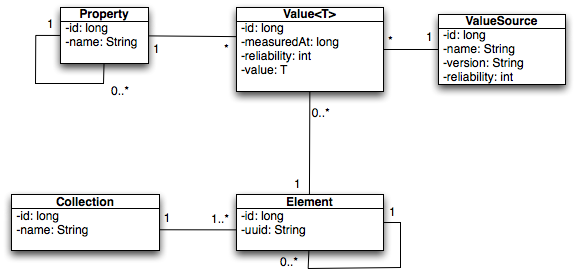
\includegraphics[width=5in]{figures/architecture/old_datamodel.png}
\caption{The data model used in the first iteration.}
\label{fig:old_datamodel}
\end{center}
\end{figure}

In the first implementation the \textit{Controller} worked in a single threaded, sequential manner due to simplicity reasons. However, preliminary experiments have shown that some tasks, such as meta data parsing make only partial use of the system resources at hand. For example the CPU utilisation was mostly less than 25\% during data parsing and storage. This was an indicator of a possible enhancement that might result in a significant speedup.

Because of the XML representation of the FITS meta data, a parser was written in order to adapt the meta data schema of FITS to the internal data model. As FITS files usually are small in size (up to 5KB), the parser that was implemented utilised a DOM based approach. Early tests over a small set of FITS XML files had feasible performance. However, the first test over larger collections revealed an issue with memory usage. Even though the amount of objects that had to be created by the DOM parser for each node in each XML document was not so high, the garbage collector of the JVM was unreliable and the overall consumption increased constantly with the XML document count and the collection size. This was in collision with the performance requirement (\textbf{R2}).

In the first iteration C3PO's persistence layer was based on the Java Persistence API\footnote{http://docs.oracle.com/javaee/6/tutorial/doc/bnbpz.html} (JPA 1.0) with Hibernate\footnote{http://www.hibernate.org/} as the persistence provider. The high-level abstraction was done via a couple of generic data access object (DAO) interfaces, which were implemented by the client application, and client modules.

This design was chosen in order to allow each client application to choose its own implementation of the persistence layer. This was important since C3PO is meant to be deployable in application server containers that support the Java EE\footnote{http://www.oracle.com/technetwork/java/javaee/overview/index.html} technology stack. For this, a special container-managed transactional model would have been needed. On the other hand, content profiling is a data intensive process which can gain from the fact that the tool can execute near the data. That is why also a local transactional model was needed, in which the tool should run locally near the data without any application server. All this would allow the separation of the data gathering and the data analysis parts of the workflow. The fact that the database is external to the tool also means that it can be setup near the data or on a specific storage sever that has enough resources at its hand to handle the load.

Using an ORM framework such as Hibernate is often very useful. However, in this instance a lot of optimisations and tweaks had to be done in order get out the most of the database. While this was certainly possible, it was not the focus of the work to fight the framework. Using JVM profiling applications revealed that a lot of resources are used during storage, because of the high volume of data. The ORM framework was the bottleneck.

In the first iteration only a prototype of the CLI application was implemented that made use of the non-transactional persistence model. It was used to measure performance and to monitor the behaviour of the whole framework. As far as the web application was concerned, only the persistence layer interfaces were implemented in order to validate the design and the separation of concerns.

Hence, the exploratory prototype revealed that this use case does not fit well into a relational paradigm and the use of an ORM framework decreased the performance of the process during storage. What is more, parsing the meta data with a DOM parser did not scale well and consumed large amounts of memory. These insights were the key to the design of the delivered prototype for C3PO.

\subsection{Second Iteration}
This section gives an overview of the implementation changes and enhancements in the second iteration and discusses the benefits and drawbacks of the alternatives.

\subsubsection{Data model}
After examination of the data at hand, it seemed that the key value structure was fitting, but through the data base normalisation, performance was compromised (\textbf{R2}). Thus, an appropriate choice was to exchange the underlying data source, which made it possible to remove the ORM framework at all. Its overhead was proven to be unnecessary during meta data adaptation and storage. Also, the analysis of the data took an unnecessary long time due to the many JOIN operations. While these could have been avoided by making the data model more specific, this would have compromised the flexibility, which was a key requirement.

For these reasons, the data model was analysed again and different storage possibilities were evaluated.  Due to the natural key-value structure of the meta data a key value store was assessed to provide a better solution to the problem. However, usually such solutions are used for caching (EHCache\footnote{http://ehcache.org}, Memchahed\footnote{http://memcached.org}, etc.) and architecture designers often have problems fitting their data model when such technologies are used for more than their purpose - caching. There are some implementations of data bases that offer most of the flexibility of the relational paradigm, high performance due to their almost key-value paradigm and out of the box horizontal scalability.

MongoDB\footnote{http://www.mongodb.org/} is a document store that uses BSON\footnote{http://bsonspec.org/} (Binary JSON) in order to store data in form of documents. 
These documents can have any kind of structure and do not have to be normalised in the relational database sense.
On top of that, MongoDB provides native facilities for executing Map Reduce \cite{Dean:2008:MSD:1327452.1327492} jobs on the server, which proved to be very useful for aggregating and filtering the data. 
As any NoSQL solution, MongoDB does not require normalised relational data.
On the contrary, NoSQL solutions give up normalisation in order to enhance the performance of specific use cases. 
MongoDB was chosen because of several reasons:

\begin{itemize}
\item \textbf{Natural fit of the data into a key-value schema.}
The data model from the first iteration was transformed into three collections (here the term collection is used in the sense of a document store and can be understood as the equivalent concept of a table in a relational database): one for the elements, one for the properties and one for the sources.
The values are embedded into each element document and thus each document represents a self-contained object with all its known meta data - values, sources and conflicts.
This has one big advantage when querying, as all values are already present without a need of joining the property table. 
Figure \ref{lst:document_structure} gives an overview of the basic structure of element documents in BSON syntax. Note that the syntax is very similar to JSON, but provides data type support (e.g. the ObjectId).

\item \textbf{Support for native Map Reduce jobs} makes it is easy to aggregate specific values of specific keys in every element document or to execute analysis queries. This enhances performance as most of the computation is done near the data.

\item \textbf{Query cursor and pagination support.}
Every query in Mongo DB returns a cursor over the data instead of the data itself. This makes navigation over the data within an application fast and efficient in terms of memory, as one does not have to consider the volume of the queried data. This lazy-loading mechanism comes in handy in numerous use cases of the application.

\item \textbf{Horizontal scaling and automatic node balancing} are supported out of the box.
This is useful when considering the amounts of data that the profiler has to deal with. It will also reduce the configuration and administration overhead if such a system is used in production.
\end{itemize}


\vbox{
\begin{lstlisting}[
caption={The structure of a C3PO element represented as a BSON document.},
label={lst:document_structure},
language={JavaScript}
]
{
	_id : ObjectId("4fe1d1c00364689befd96b62"),
	name: "MyObject",
	uid: "/some/unique/identifier/within/the/source",
	collection: "MyCollection",
	metadata: {
		key_one : {
			status : "OK",
			value: "some value",
			sources :  ["..."]
		},
		key_two : {
			status : "OK",
			value: "other value",
			sources:  ["..."]
		}
	}
}
\end{lstlisting}
}

\subsubsection{Core}
In the second iteration, the \textit{Controller} and the meta data adaptors were implemented again following a master-worker pattern.
The Controller uses the \textit{Gatherer} interface to traverse the raw meta data files and spawns an adaptor worker thread for each file that has to be processed. This change resulted in much larger utilisation of CPU resources. Each meta data adaptor runs in a thread and is responsible for parsing meta data files that conform to a specific meta data schema. The C3PO prototype makes use of a single adaptor for the FITS output format as described in Section \ref{lbl:tool_support}. 

The parser implementation of the FITS adaptor was also changed due to the previous performance results. This time, a SAX based approach was used. The Apache Commons Digester library\footnote{http://commons.apache.org/digester/} provides a special SAX parser that traverses each document only once and does not require the building of a complex DOM tree. This results in a much faster parsing with significantly less memory resources.

\subsubsection{Applications}
The CLI application was modified so that it reflects the changes of the new persistence layer. This allowed for faster and easier processing near the data (\textbf{R1}).

Since the underlying technology stack was different and there was no need of transactional persistence model a new approach was also chosen for the web application. It makes use of a popular web application framework, called PlayFramework\footnote{http://playframework.org}, which does not rely on a complex technology, such as EJBs. It supports the developer to follow the MVC pattern and allows the rapid development of a REST \cite{Fielding:2000:ASD:932295} interface. REST was chosen for two main reasons. For one, it is easy to understand and pretty straightforward to implement. This allows easy integration with other tools such as monitoring services and a variety of client applications. The second reason is that other technologies such as JavaServer Faces Technology\footnote{http://www.oracle.com/technetwork/java/javaee/javaserverfaces-139869.html} (JSF) and Enterprise Java Beans Technology\footnote{http://www.oracle.com/technetwork/java/javaee/ejb/index.html} (EJB) would have meant that only a few application servers would be compliant and able to support the application.
%REST cite: http://www.ics.uci.edu/~fielding/pubs/dissertation/rest_arch_style.htm

The UI was implemented with the help of the framework, by utilising Scala\footnote{http://www.scala-lang.org} templates and standard technology such as HTML5, Javascript and CSS3. It enables the user to select her collection and obtain a deeper overview by filtering the data based on specific properties and values as shown in Figure \ref{fig:web_app_overview}. The screenshot shows the overview page of a real world collection. It shows the distributions of seven properties: mime type, format, format version, validity, well-formedness, creating application and created date. In the upper right corner of the overview, the application provides statistical information about the size of the objects (\textbf{R4}). Although it is not possible to see from the screenshot, the diagrams are interactive and give the user the possibility to filter the data based on any measure (\textbf{R5}). From the navigation bar in the top, one can see that C3PO also has features for browsing the objects, finding representative sample records and exporting data (\textbf{R3}).

\begin{figure}[tbp]
\begin{center}
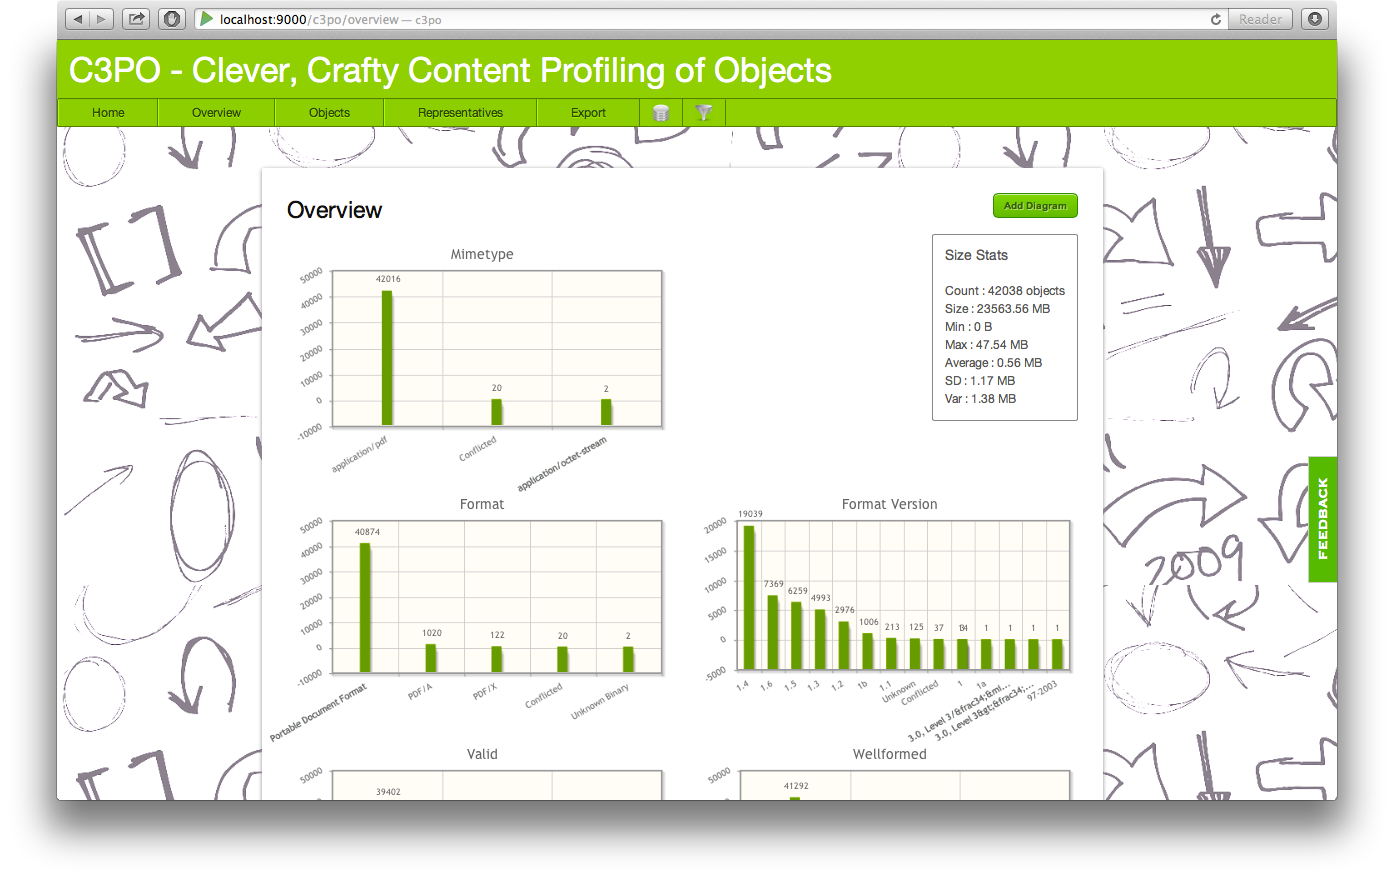
\includegraphics[width=5.5in]{figures/architecture/web_app_overview}
\caption{Screenshot of C3PO - Overview of a collection.}
\label{fig:web_app_overview}
\end{center}
\end{figure}
\clearpage

\subsection{Comparison and Results}
Due to the changes made in the second iteration significant performance and scalability optimisations were achieved.

Table \ref{tab:iterations_performance_metrics} shows the average time needed by C3PO for processing 1000 FITS files in each of the two iterations. This includes traversing, reading in the data, parsing it and storing it within the data store. All of these experiments were conducted on a single commodity machine.

The collections used are from real world preservation scenarios. Both are significant in size, where the first consists of about 42 thousand PDF documents and the second consist of about 550 thousand web harvested material. The processing includes the time for parsing, converting to the internal data model and storing to the data base. Both experiments are conducted on the same common hardware.

The first implementation needed 350 seconds per thousand FITS files on average for the PDF collection and didn't finish due to memory issues for the web collection. In the second iteration the memory issues were resolved and the DOM parser was exchanged by a SAX parser, which resulted in 80 seconds per thousand files on average for the document collection and 98 seconds per 1000 files for the web data. After the removal of the ORM and some further optimisations in the SAX parsing approach a significant boost was achieved; the PDF collection was processed with a rate of 3 seconds per thousand files and the Web data with 2 seconds per thousand files.

\begin{table}[h]
\centering
\begin{tabular}{l || c | c | c}
\hline
\multirow{2}{*}{\textbf{Collection}} &  \textbf{1. Iteration} & \multicolumn{2}{c}{\textbf{2. Iteration}} \\
                    & \textbf{DOM + ORM} & \textbf{SAX + ORM} & \textbf{SAX + Mongo} \\
\hline
PDF collection & 350 sec  & 80 sec & 3 sec \\
\hline
Web collection & threw exception & 98 sec & 2 sec \\
\hline
\end{tabular}
\caption{C3PO's average processing time of 1000 files in two different collections}
\label{tab:iterations_performance_metrics}
\end{table}

The process parallelisation improved the speed even more. Table \ref{tab:parallel_performance_metrics} shows
more than 30\% speedup for processing the whole govdocs1 collection, which consists of about 1 million FITS files of mixed data.

\begin{table}[h]
\centering
\begin{tabular}{l || c | c}
\hline
\textbf{Collection} & \textbf{1 Thread} & \textbf{8 Threads} \\
\hline
govdocs1 & 165 min & 104 min \\
\hline
\end{tabular}
\caption{C3PO's processing time of the govdocs1 collection with one and 8 worker threads}
\label{tab:parallel_performance_metrics}
\end{table}

Furthermore, exporting a sparse matrix of all property values for every element in the collection was shown to be much faster. This was due to the fact that the internal representation of the data needed no JOINS anymore and can be done by single iteration over a database cursor.

Many of the analysis queries were changed to be done by map-reduce jobs. Since these run near the data and not in the application itself, the scalability of such queries was significantly improved.

Chapter 5 summarises detailed performance measures of the govdocs1 and a web archive collection as well as the time needed for profile generation and matrix export and gives an overview of the capabilities of the tool.

\subsection{Interfaces and Extension Points}
In order to extend the system, the framework provides a couple of interfaces. One important extension point for later use is the \textit{GathererInterface} which provides an abstraction for the source of the raw meta data. It exposes a unified interface allowing the \textit{Controller} to obtain streams to the next N files that have to be processed. This design allows a transparent view to the other modules in the system. The prototype of C3PO provides an implementation only for local file systems. However, extending it to fetch data from a different source is just a matter of implementing a single interface, which is able to count the files to be processed and to open streams to the next N files. It is up to the implementing class to decide, whether the data will be retrieved over the network and the stream will be passed directly for further processing or it will be cached in batches to the local file system. Depending on the use case both could make sense and thus it is left in the responsibility of the service provider.

Clearly, meta data representation is another important aspect in such as system. For the prototype, FITS was chosen due to it benefits regarding normalisation and conflict detection. Nonetheless, other formats can make sense in specific use cases and when integrating with different sources, that utilise different meta data schemas. In order to extend C3PO, one has to implement a simple adaptor that is able to parse the new schema and return the data in a way that fits C3PO's data model. A drawback here is that this will potentially break the property normalisation. For example, two different meta data schemas can have two different property names with the same semantical meaning. There are a couple of solutions to this problem, which are taken into account in the design, but are not implemented due to insufficient information of real world scenarios. The first could be to provide the mapping between these colliding properties via some user configuration and to take them into account during parsing or post-processing. The second solution would be to allow the usage of a single adaptor based on the use case.

In order to obtain a profile, client applications can use the REST API. With a few simple calls, a XML representation of a collection profile can be generated and retrieved. This file conforms to the proposed schema in Chapter 3 and provides simple aggregations of the data.
 
\section{Representative Sets}
Representative sets are one of the most important features of C3PO, as they provide the basis for experiments during the planning phase. The selection of valid representatives can influence the decisions of a planner for the future of specific content strongly. There are many different ways of selecting a small set of representatives.
Here we present a few algorithms that were implemented and discuss their benefits and drawbacks. It is important to keep in mind that real world scenarios can involve large collections of thousands to millions and even more digital objects, but usually the experiments during preservation planning are done on a very small set of representative sample objects in the order of 10 objects.

In the following, we present only the core of the algorithm and leave out some basic input checks, such as the initial size of the collection or the filtered subset, etc.

\subsection{Random Selection}
As the  name suggests, this algorithm takes N random elements from the larger set and returns them. A simple pseudo code implementation looks like Algorithm \ref{alg:random_selection}. Unfortunately, this approach is widely used in real world scenarios, due to the lack of automation support and understanding of the content at hand. One drawback of this approach is that it will most probably provide terrible results when applying it on highly heterogeneous content.
Nonetheless it could be useful in some cases, if the content is first filtered. For example, one can first apply some filters with C3PO and split the collection into smaller sets that are homogeneous with respect to certain properties and then apply this algorithm on each of the subsets. If the smaller subsets are homogeneous enough, it is possible to achieve good results. Nonetheless, splitting and analysing the content could potentially take a lot of time.

\begin{algorithm}[!htb]
\SetKwFunction{RSS}{Random Sample Selection}
\SetKwInOut{Input}{Input}
\SetKwInOut{Output}{Output}

 \Input{A set of digital objects S and a upper limit N for the sample objects set}
 \Output{A set of random representative sample objects R}
 \BlankLine

\tcp{gets the number of objects in S}
 count = \textit{S.size()}\; 
 
 \While{R.size() $<=$ N} {
   \tcp{gets a pseudo random number between 0 and count}
   rand = getRandomNumber(count)\;
   \tcp{S[rand] get the object at index 'rand'}
   sample = S[rand]\;
   \tcp{add() appends the object to R}
   R.add(sample)\; 
 }
 
 \caption{Random sample selection}
 \label{alg:random_selection}
\end{algorithm}

\subsection{Size Statistics}
This approach is probably the most common approach currently used by planners and preservation experts. It also selects random elements, however it considers some statistical information regarding the size of objects. This decision stems from the observation that preservation action tools often perform badly on objects with a large variation in size. Thus planners often take the smallest, largest and several average-sized objects and conduct the experiments over them. If there are no other significant variations and differences in the objects, the selected representative set, could provide good results for planning. However, if the objects have significant variations in characteristics, other than the size that might influence the preservation action tools and the algorithm would be error prone.

A possible pseudo code implementation is provided in Algorithm \ref{alg:size_selection}. As this algorithm makes use of the standard deviation in order to find objects of size near the average size, it utilises an implementation of another online parallel algorithm for calculating the variance of a set of data. An online algorithm is one that operates on the data without having all needed input from the beginning. This particular calculation of the variance in a single pass over the data was suggested by West in \cite{West:1979:UMV:359146.359153} and is a parallel algorithm that takes into account a sum of weights at each step. Listings \ref{lst:map_function} to \ref{lst:finalize_function} show the map, reduce and finalize functions (in JavaScript notation) of a Map Reduce job that implements West's algorithm.

This approach is slightly better than the previous one, as it considers at least one characteristic of the meta data, that indeed often has influence on the experiments. If applied on a homogeneous set (with respect to the digital object type), it could give good results. Nonetheless, there are other factors that have to be considered, especially in cases where the variance of the size in the collection is small.

\begin{algorithm}[bh]
\SetAlgoLined
\SetKwFunction{SSS}{Size Statistics Sample Selection}
\SetKwInOut{Input}{Input}
\SetKwInOut{Output}{Output}

 \Input{A set of digital objects S and an upper limit N for the sample objects set}
 \Output{A set of random representative sample objects R}
 \BlankLine

\tcp{gets the number of objects in S}
count = \textit{S.size()}\; 

\tcp{map reduce job that calculates}
\tcp{ statistics for the property 'size'}
stats = numericMapReduceJob('size')\;
min = stats.min\;
max = stats.max\;
avg = stats.avg\;
sd = stats.sd\;
low = floor(avg - sd / 10)\;
high = ceil(avg - sd /10)\;
\BlankLine
minObj  = querySize(min)\;
maxObj = querySize(max)\;
A = querySizeBetween(low, high)\;
\BlankLine
R.add(minObject)\;
R.add(maxObject)\;
\BlankLine
  \While{R.size() $<$ N} {
    R.add(A.remove(0))\;
  }
 \caption{Size Statistics Sample Selection}
 \label{alg:size_selection}
\end{algorithm}


\vspace{1em}
\begin{lstlisting}[
caption={The Map function for basic statistical aggregations.},
label={lst:map_function},
language={JavaScript}
]
function map() {
  var size = this.metadata['size'].value;
  emit(1,
  	{sum: size, 
	 min: size,
	 max: size,
	 count:1,
	 diff: 0,			// sum of squares of differences from the (current) mean; sum((val-mean)^2)
   });
}
\end{lstlisting}


\begin{lstlisting}[
caption={Th Reduce function for basic statistical aggregations.},
label={lst:reduce_function},
language={JavaScript}
]
function reduce(key, values) {
  var a = values[0]; 		// will reduce into a
  for (var i = 1; i < values.length; i++){
    var b = values[i];		// will merge b into a
    var delta = a.sum / a.count - b.sum / b.count;		// a.mean - b.mean
    var weight = (a.count * b.count) / (a.count + b.count);
    
    a.diff += b.diff + delta * delta * weight;
    a.sum += b.sum;
    a.count += b.count;
    a.min = Math.min(a.min, b.min);
    a.max = Math.max(a.max, b.max);
  }
  return a;
}
\end{lstlisting}

\begin{lstlisting}[
caption={The Finalize function for basic statistical aggregations.},
label={lst:finalize_function},
language={JavaScript}
]
function finalize(key, value){
  value.avg = value.sum / value.count;
  value.variance = value.diff / value.count;
  value.stddev = Math.sqrt(value.variance);
  return value;
}
\end{lstlisting}

\subsection{Systematic Sampling}
Systematic sampling is an optimisation of the random approach and is an equal-probability method. In other words, it is fairer as every object in the set has equal probability to be chosen as a representative. It divides the content into \textit{n} buckets and calculates a \textit{skip} variable by dividing the number of objects in the population \textbf{N} by the number of buckets \textbf{n}. Then a random starting point is chosen between \textit{zero} and the calculated \textit{skip}. Afterwards, adding the \textit{skip} to the index of the last chosen element chooses the next \textit{n-1} elements.  This will result in one element per bucket.

Even though this method is fairer, it still shows the same problems as the random sample selection algorithm. A pseudo code implementation is given in Algorithm \ref{alg:systematic_sampling}

\begin{algorithm}[!htb]
\SetAlgoLined
\SetKwFunction{SSS}{Systematic Sampling Selection}
\SetKwInOut{Input}{Input}
\SetKwInOut{Output}{Output}

 \Input{A set of digital objects S and an upper limit N for the sample objects set}
 \Output{A set of random representative sample objects R}
 \BlankLine

\tcp{gets the number of objects in S}
 count = \textit{S.size()}\; 
 
 limit = round(count / N)\;
 \tcp{generates a random number with a upper limit}
  skip = nextRandom(limit)\;
  
  \While{R.size() < N} {
     offset = skip * R.size() + skip\;
     R.add(S[offset])\;
  }
 \caption{Systematic Sampling Selection}
 \label{alg:systematic_sampling}
\end{algorithm}

\pagebreak
\subsection{Distribution Coverage}
The distribution coverage algorithm tries to find sample objects with the same distribution of the property value pairs of characteristics chosen by the planner. For example, if there is a collection consisting of \textit{40\% PDF documents} and \textit{40\% Word documents} and \textit{20\% other documents}, the desired sample set size should be ten and the chosen property is \textit{format}, then the algorithm will select four \textit{PDF files}, four \textit{Word} files and two other files at random that are not PDF or Word documents.
If the planner also wants another property value distributions taken into account, then these are considered by building all possible key-value pairs. The algorithm tries to find the nearest distribution possible over all the combinations of the selected properties and their values.
Continuing the previous example, If a planner wants to consider also the property \textit{format version} and the collection has documents with versions \textit{1.2} and \textit{1.4} for PDF as well as \textit{2003} and \textit{2007} for the Word documents, then the algorithm will find all possible combinations \textit{(PDF - 1.2, PDF - 1.4, PDF - 2003, PDF - 2007, Word - 1.2, Word - 1.4, Word - 2003, Word - 2007 etc. )}. Afterwards the occurrences for each combination in the data set will be counted and the approximate distribution will be returned. This means that the number of combinations is equal to the product of the distinct value occurrences for each property. In this example, two distinct occurrences for the property \textit{format} and four distinct occurrences for the property \textit{format version} equals eight combinations. Obviously some of the combinations will always return zero, as there is no such format as \textit{Word - 1.4}. 

This can be avoided if enough information about the correlation of the different properties is provided. As this is not the focus of this thesis, the current version of the algorithm builds all possible combinations and does not consider the correlation between properties.

Algorithm \ref{alg:distribution_coverage} presents a simple pseudo implementation. It takes a set of digital objects S, an upper limit for the samples set and a set of properties P.

In a first phase a simple multi-dimensional array (matrix) is build. It goes over all passed properties and their distinct value occurrences. In order to populate it the algorithm obviously needs to issue database queries (line 5) or receive the distinct property value pairs as input.

In a second phase, it creates all possible combinations of the property value pairs as in the example above. Each combination consists of one value per property and the count of objects that have these exact values for the given properties. In the next step the combinations are sorted based on count.

Afterwards the algorithm iterates over the combinations until the size of the set of sample objects R is smaller than 'N' and calculates the ratio of count of objects in each combination and the total collection size. It issues a query to collect a number of objects that have the same ratio in the sample set R as the ratio within the collection.

This algorithm is better with respect to heterogeneity of properties within the same digital object type. A planner that makes use of it has to understand that the algorithm does not consider the long tail of files. It is suggested, that these
are handled separately, as they are often responsible for messed up experiment results.

Nonetheless, the selection of a larger set of properties could impede the performance and the validity of the results, as the occurrences for each combination of property and values will get significantly smaller. Thus a planner has to consider carefully, which combinations of properties make more sense.

\begin{algorithm}[!htb]
\SetAlgoLined
\SetKwFunction{SSS}{Distribution Coverage Selection}
\SetKwInOut{Input}{Input}
\SetKwInOut{Output}{Output}

 \Input{A set of digital objects S, an upper limit N for the sample objects set and a set of properties P}
 \Output{A set of random representative sample objects R}
 \BlankLine

\tcp{creates a matrix M with the properties and all distinct values for each property}
M[P.size()][]\;

i=0\;
\ForEach{property $p$ of $P$}{
  j=0\;
  \tcp{issues a database query}
  DV = findDistinctValuesForProperty( P )\;
  V[DV.size()]\;
  \ForEach{value $dv$ of $DV$} {
    \tcp{PV is property value pair wrapped in an object}
    V[j] = PV(p, dv)\;
    j = j+1\;
  }
  M[i] = V\;
  i = i + 1\;
}

\tcp{C is a list of combinations over all property value pairs}
\tcp{A combination is a wrapper object that has a distinct value for each property and the count of objects that
conform to the combination}
\tcp{The size of the combinations equals the product of the size of distinct values for each property}
C =  combinations( M )\;
\tcp{sort based on count}
sortDescending( C )\;

 \ForEach{combination $c$ of $C$} {
 
  \If{R.size() $<$ N} {
   percent = c.count() * 100 / S.size()\;
   tmpLimit = round(percent / 100 * N)\;
   
   \tcp{get maximum 'tmpLimit' objects out of S that conform to the current combination}
   R.addAll(getObjectsConformingToQuery(c.query(), tmpLimit))\;
   }
}

return R\;

 \caption{Distribution Coverage Sample Selection}
 \label{alg:distribution_coverage}
\end{algorithm}

\section{Future Points of Interest}
There are many topics that can be handled and implemented in future work. Here we outline some and briefly discuss them:
\begin {itemize}
\item \textit{Scalability} is very important, as the volumes of data will grow more and more over time. Even though the hardware resources and provided performance also grow over time the issue of scalability is very important. The author believes that horizontal scalability is the best way to pursue. The current design decisions follow that path. More specifically, future enhancements should include distributed map-reduce jobs and the caching of specific results, which will enhance the systems responsiveness.

\item \textit{Continous Profiling} is important as collections change over time. The support for including meta data of new and changed objects as well as adapting the computed aggregations in a easy, fast and scalable fashion is critical for the success of such an application in production use. Thus the investigation of the problems that arise with this will be important for future versions of the tool. The Map-Reduce facilities provide a potential solution to such a problem. In contrast to SQL solutions, here it is possible to aggregate new data and reuse old results, which are then just merged as the reduce function is always the same.

\item \textit{Input to Digital Preservation Tools}. Monitoring systems and simulators enhance the preservation planning processes by providing relevant and trustworthy information that is often hard to obtain due to its distribution and by offering simulations and projections of different outcomes based on current decisions and policies. Such systems heavily rely on larger amount of data. Integration with a content profile tool will play an important role for such tools as well as preservation planning activities.

\item \textit{Representative Sets} are the foundation for unbiased experiments and thus better performing algorithms in terms of speed and effective selection should be the focus of future work as well. 

\item \textit{Visualisation and Interactivity}. A wider variety of visualisations of different aspects of a collection can help and influence the decision of a user.
\end{itemize}

\section{Integration}
The prototype was integrated with two digital preservation systems developed within the SCAPE project. Here we shortly describe the concept of the integration, why it makes sense and how it contributes towards a full implementation of the presented preservation planning environment in Chapter 3.

\subsection{Scout - A preservation monitoring system}
As preservation planning is a continuous process that has to be repeated constantly, the preservation environment
foresees a special component that monitors certain types of changes in characteristics that are of interest to a planner.
Monitoring is responsible for the detection of important events such as new emerging formats, new software or new versions of software, but also violation of institutional policies and many more. 
One of the important aspects that a monitoring component has to follow is the content profile. Doing so, it can cross match the formats within the profile with formats present in registries and institutional objectives. For example, an institution might have an objective that all image content within a repository has to have lossless compression.

As C3PO exposes a REST interface for generating and retrieving a profile in XML format, integration between the SCAPE monitoring Service - Scout, and C3PO was created. Scout contacts the profiler over the REST API and periodically fetches a profile for each known collection. Afterwards the profile is parsed and the values of specific properties such as size, format distribution, etc. are collected.

If a planner has created specific conditions or constraints within Scout and these are met or violated after the new values are measured, then the planner will be notified and will potentially have to change the current plan for a given collection.

\subsection{Plato - A preservation planning suite}
A huge part of the planning environment is covered by the preservation planning tool - Plato.
Plato supports a planning expert through all phases of the planning process, from plan creation to building an executable plan .

Up until the third version of Plato, a planner had to define the scope of every new plan by hand. This implied that the definition of the preserved collection was done manually. As this is a tedious process, planners often provide only high-level descriptions of the collection and also select all sample objects randomly.

Throughout the SCAPE project, C3PO was integrated with Plato in order to semi-automatically define the scope of a plan not only in a high level assertion, but also in more detail, providing a correct format distribution and more.
Allowing a planner to filter a collection and export an XML profile via C3PO enables the expert to easily start creating new plans, without having to manually inspect the type of the objects and find representative.

After the exported profile is uploaded to Plato, the tool parses it and fills in all necessary information. Moreover, the sample records information is filled automatically and the used algorithm is provided in order to have evidence later on.
As every object known to C3PO has a unique identifier (within its source), Plato can check where the collection comes from. If the source is known and the user provides the correct credentials, Plato automatically downloads the sample objects for the experiments during the following steps.
Having a list of object identifiers that are part of the collection has also another advantage. After a plan is build and ready for execution, Plato can reopen the stored profile and read out all identifiers that are part of the collection. These are included within the executable plan. This has the advantage that once the executable plan is fed back to the source (repository) for execution, the repository automatically knows on which objects it has to apply the executable actions defined in the plan.

\subsection{Observation}
This rather simple integration of profiling with the two larger components of the preservation environment  enhances the experience of a planner greatly. A preservation expert does not only benefit from the automation support provided by the profile, but also from the fact that now he can do a complete preservation lifecycle of a collection. To illustrate this example, consider the following scenario. In a first step the institutional policies define that objects within the repository have be covered with a plan. An expert creates a profile with C3PO and uploads it to Plato. Plato automatically defines the scope of the plan, fills in the sample objects and automatically fetches them from the repository. The expert defines and conducts the experiments with help of Plato. After that a recommendation is chosen and an executable plan is created. This plan is deployed within the repository and gets executed. Meanwhile a monitoring component observes the profile of the repository as well as the operations of the execution and notifies the planning expert when certain changes or potential problems occur.
